V poslednej časti práce prezentujeme praktické výsledky našej implementácie CR-indexu.
% co variujeme, co s cim porovnavame atd

\section{Testovacie prostredie}
Všetky testy prebiehali pod 64-bitovou verziou operačného systému Linux verzie 3.16.0-34. Testy boli kompilované kompilátorom \texttt{gcc} verzie 4.9.1 s prepínačmi \texttt{-std=c++11} a \texttt{-O3} a spustené na hardvéri s CPU \texttt{Intel(R) Core(TM) i7-4910MQ CPU @ 2.90GHz} a 16GB RAM. Na meranie spotreby pamäte a rýchlosti odpovedania na dotazy sme použili testy \texttt{benchmark/construct.cpp} a \texttt{benchmark/query.cpp} popísané v časti \ref{sec:vonkajsia_struktura}.

\subsection{Testovacie dáta}
\subsubsection{Sady readov}
Sady readov sme generovali z genómu baktérie \emph{Staphylococcus aureus}\footnote{Dostupné na internete na stránke \url{http://gage.cbcb.umd.edu/data/index.html}}\footnote{Z genómu na stránke sme odstránili genómy plasmidov a použili len genóm samotnej baktérie.}. Tento genóm má dĺžku 2872915 báz, dĺžku readu $l$ sme zvolili 100 a dĺžku dotazu $k=13$. 

% tabulku asi
Podľa týchto parametrov sme dorátali, že počet readov v sadách pre jednotlivé pokrytia je: 57458 readov pre pokrytie $2\times$, 143645 readov pre pokrytie $5\times$, 287291 readov pre pokrytie $10\times$, 574583 readov pre pokrytie $20\times$ a 1436457 readov pre pokrytie $50\times$.

V poslednom teste sme použili reálnu, nie generovanú sadu readov. % odkial + samplovanie

\subsubsection{Sada dotazov}
% nahodne vs. generovane z genomu/readov

\section{Testy}

\subsection{CR-index vs GkArray}
% pamat
% variovat coverage (a/alebo error rate)

\subsection{CR-index vs GkArray 2}
% query time
% variovat coverage (a/alebo error rate)

\subsection{Pamäť vs. pokrytie}
V tomto teste sme merali závislosť spotreby pamäte na pokrytí pre rôznu chybovosť readov. 

\begin{figure}[h]
    \centering
    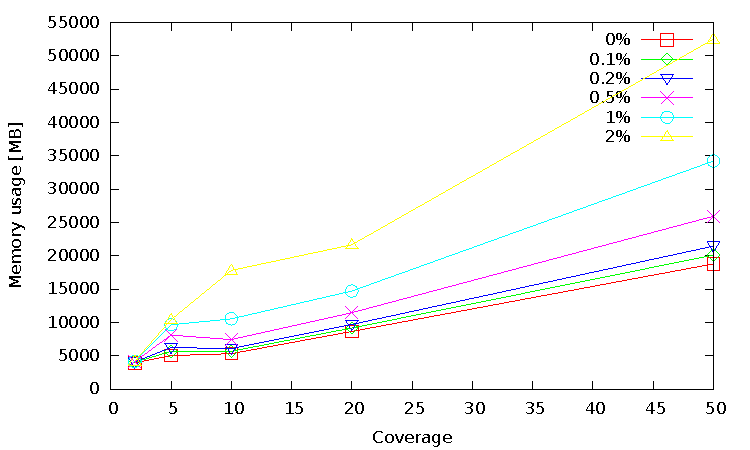
\includegraphics[width=16.5cm]{staphyl}
    \caption{Závislosť spotreby pamäte na pokrytí pre rôznu chybovosť vstupnej sady readov.}
    \label{fig:graf_staphyl}
\end{figure}

\subsection{Test na reálnych dátach}
% graf realne data, variujem coverage (samplovanim nasimulujem ine converages)

\section{Zhrnutie a interpretácia výsledkov}

\todo{nekonzistentnost oznaceni, superstring je raz ss a raz S}\\
\todo{zmenit \emph{ready} na ready} \\
\todo{usamova minimovka - citacie} \\
\todo{usamova minimovka - 1.1 shortest common superstring je np-hard + 2.5 apx.(?)} \\
\todo{mensie odstavce} \\
\todo{vyhodit slovo 'nejak'}